\documentclass[../main.tex]{subfiles}
\externaldocument{clustering_methods}


\begin{document}

\section{Neural Networks} \label{Neural Networks}

\subsection{Introduction}
On the most basic level neural networks consist of many simple models (e.g. linear and logistic models) that are chained together in a directed network. The models sit on the neurons (nodes) of the network. The most important components of neurons are:
\begin{enumerate}
    \item \textbf{Activation}: $a = Wx+b$ ($W$ = weights and $b$ = bias)
    \item \textbf{Non-linearity}: $f(x, \theta)=\sigma(a)$ (e.g. a sigmoid function for logistic regression, giving you a probability output. $\theta$ is a threshold)    
\end{enumerate}
The neurons (nodes) in the first layer uses as its input the sample values and feeds its output into the activation function of the next nodes in the next layer, a.s.o. The later layers should thereby learn more and more complicated concepts or structures. 

\begin{figure}[h]
    \centering
    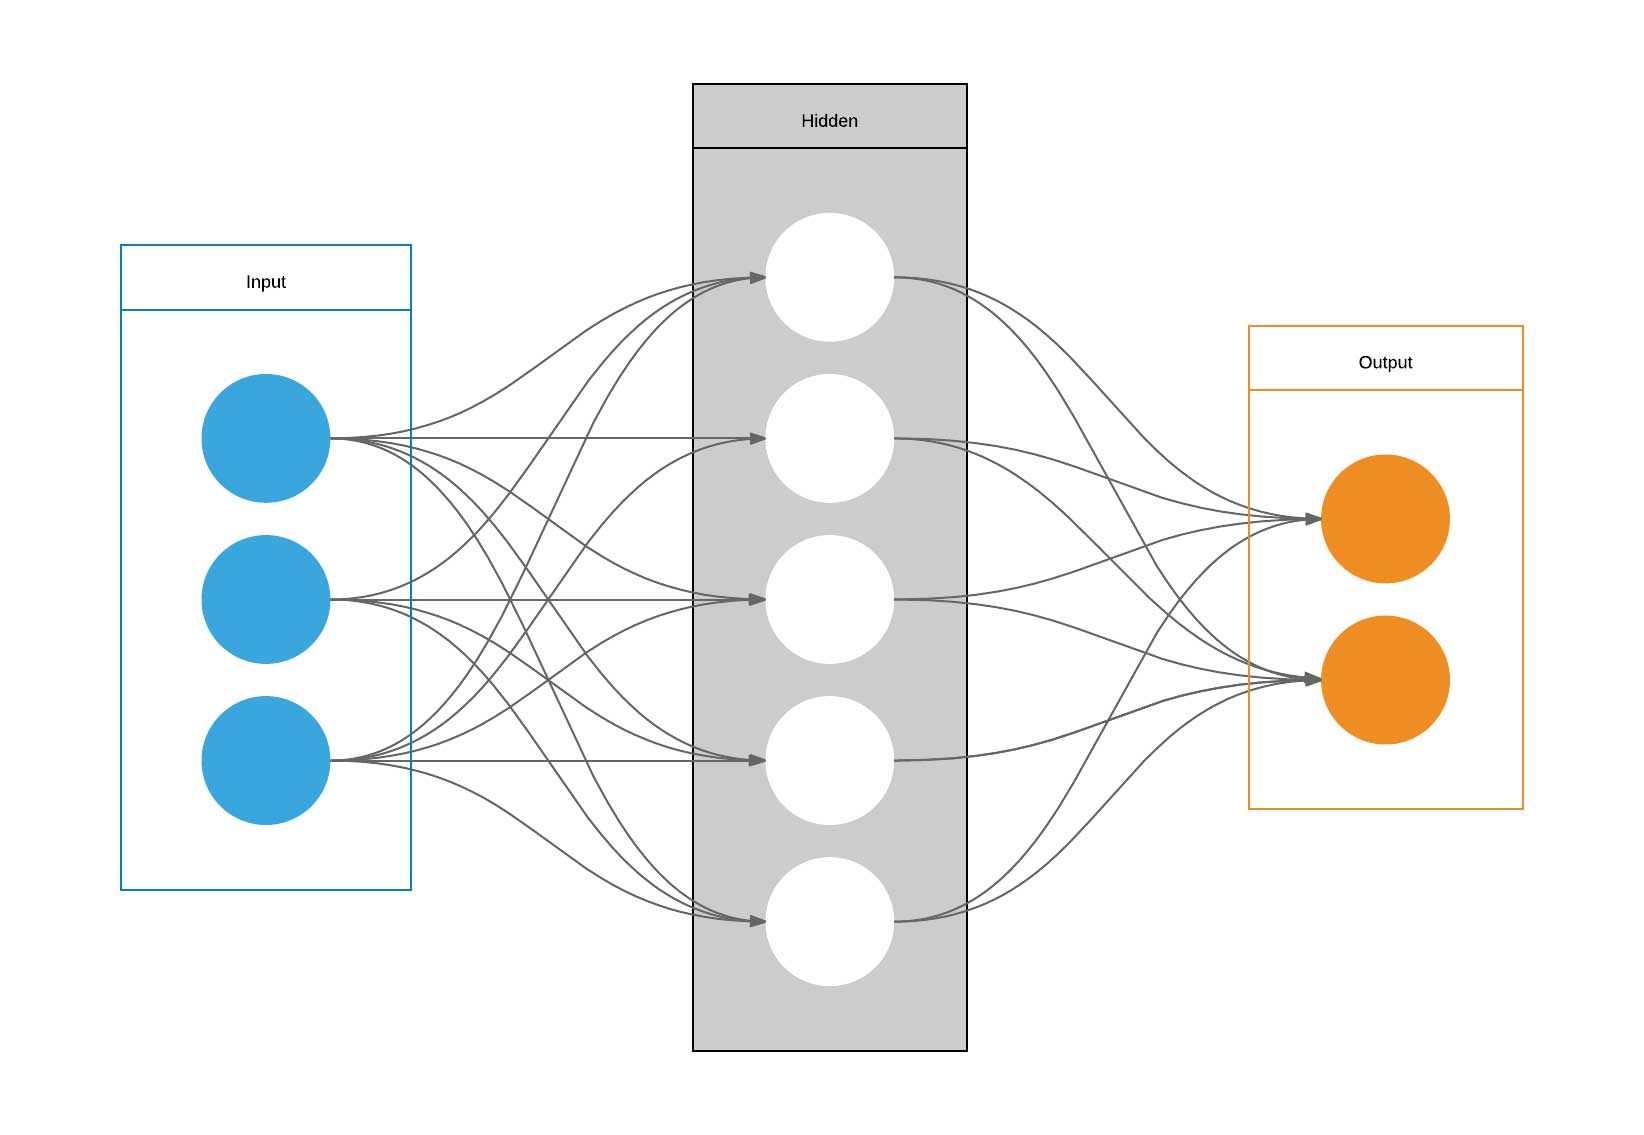
\includegraphics[width=0.7\textwidth]{../figures/Artificial_Neural_Network.jpg}
    \caption{Model of an artificial neural network with one hidden layer. \textit{Figure from \href{https://commons.wikimedia.org/wiki/File:Artificial_Neural_Network.jpg}{user LearnDataSci on wikimedia.org}.}}
    \label{CDF}
\end{figure}

\subsubsection{Non-Linearities}
Different non-linear functions can be used to generate the output of the neurons. 
\paragraph{Sigmoid/Logistic Functions}

\paragraph{Tanh Functions}

\paragraph{Rectifiers/ReLU}



\paragraph{Terminology}
\begin{itemize}
    \item [] \textbf{Input layer/visible layer:} Input variables
    \item [] \textbf{Hidden layer:} Layers of nodes between input and output layer
    \item [] \textbf{Output layer:} Layer of nodes that produce output variables
    \item [] \textbf{Size:} Number of nodes in the network
    \item [] \textbf{Width:} Number of nodes in a layer
    \item [] \textbf{Depth:} Number of layers
    \item [] \textbf{Capacity:} The type of functions that can be learned by the network
    \item [] \textbf{Architecture:} The arrangement of layers and nodes in the network
\end{itemize}

\subsection{Feedforward Neural Network / Multi-Layer Perceptron}
This is the simplest type of proper neural networks. Each neuron of a layer is connected to each neuron of the next layer and there are no cycles. 
The outputs of the previous layer corresponds to the $x$ in the activation function. Each output ($x_i$) of the previous layer gets it's own weight ($w_i$) in each node and a bias ($b$) is added to each node. Neurons with a very high output are "active" neurons, those with negative outputs are "inactive". The result is mapped to the probability range by (commonly) a sigmoid function. The output is then again given to the next layer. \\
\attention If your input layer has 6400 features (80*80 image), a network with 2 hidden layers of 16 nodes will have $6400*16+16*16+16*10+16+16+10 = 102'858$ parameters. This is a very high number of degrees of freedom and requires a lot of training samples.

\begin{tcolorbox}[title=Implementation of Feedforward Neural Nets]
    \begin{lstlisting}
        from torch import nn

        class CustomNet(nn.Module):
            def __init__(self):
                super(CustomNet, self).__init__()
                self.lin_layer_1 = nn.Linear(in_features=10, out_features=10)
                self.relu = nn.ReLU()
                self.lin_layer_2 = nn.Linear(in_features=10, out_features=10)
        
            def forward(self, x):
                x = self.lin_layer_1(x)
                x = self.relu
                x = self.lin_layer_2(x)
                return x
        
            def num_flat_features(self, x):
                size = x.size()[1:] # Use all but the batch dimension
                num = 1
                for i in size:
                    num *= i
                return num 
        
        new_net = CustomNet()
        \end{lstlisting}
\end{tcolorbox}

\subsubsection{Bekpropageshn} \index{Back propagation}
This is the method by which neural networks learn the optimal weights and biases of the nodes. The components are a cost function and a gradient descent method. \\
The cost function analyses the difference between the designated activation in the output layer (according to the label of the data) and the actual activation of that layer. Commonly a residual sum of squares is used. \\ You get the direction of the next best parameter-combination by using a \textit{stochastic gradient descent} algorithm using the gradient for your cost function:
        \begin{enumerate}
            \item We use a "mini-batch" of images for each round/step of the gradient descent. 
            \item We calculate squared residual of each feature of the output layer for each sample.
            \item From that we calculate what the bias or weights from the output layer and the activation from the last hidden layer must have been to get this result. We average that out for all images in our mini-batch.
            \item From that we calculate the weights, biases and activations of the upstream layers $\rightarrow$ we \textit{backpropagate}.
        \end{enumerate}




\subsection{Convolutional Neural Networks}

\subsection{Autoencoders}
Contrary to the other architectures, autoencoders are used for unsupervised learning. Their goal is to compress and decompress data to learn the most important structures of the data. The layers therefore become smaller for the encoding step and the later layers get bigger again, up to the original representation of the data. The optimization problem is now: 
\begin{equation}
    \min_{W,b} \frac{1}{N}*\sum_{i=1}^N ||x_i - \hat{x}_i||^2
\end{equation}
with $x_i$ being the original datapoint and $\hat{x}_i$ the reconstructed datapoint. 

\begin{figure}[h]
    \centering
    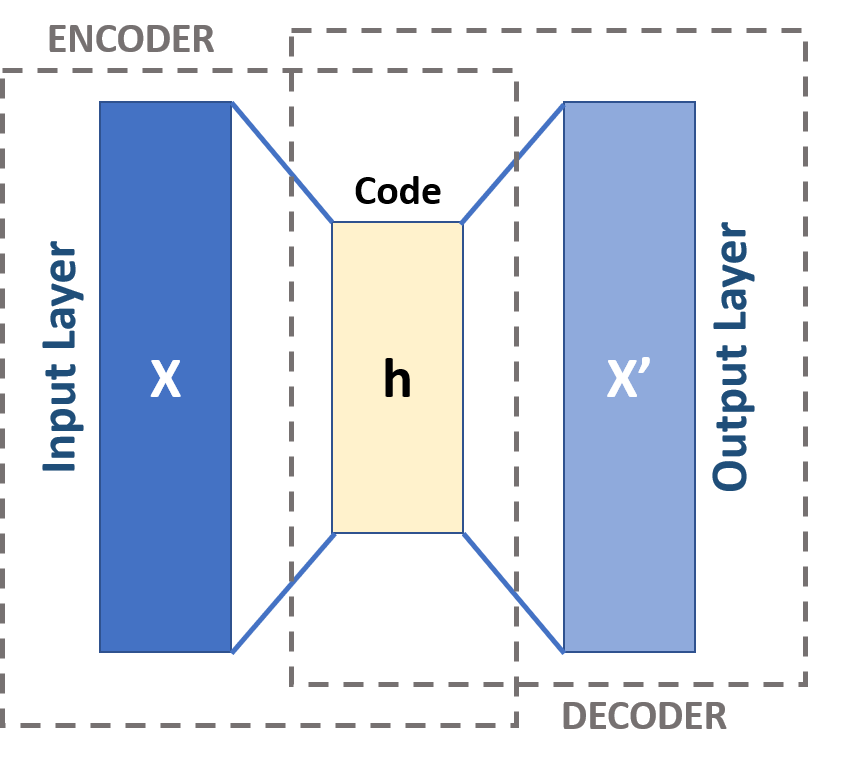
\includegraphics[width=0.5\textwidth]{../figures/Autoencoder_schema.png}
    \caption{Model of an autoencoder. The encoder layers compress the data towards the code layer, the decoder layers decompress the data again. \textit{Figure from \href{https://commons.wikimedia.org/wiki/File:Autoencoder_schema.png}{Michela Massi on wikimedia.org}.}}
    \label{CDF}
\end{figure}

\subsubsection{Autoencoders for clustering}
    You can look at layers of a NN as ways to represent data in different form of complexity and compactness. The code layers of autoencoders are a very compact way to represent the data. You can then use the compressed representation of the code layer and do clustering on that data. Because the code layer is however not optimized for that task XXXX combined the cost function of the \textbf{autoencoder and k-means clustering}: 
    \begin{equation}
        \min_{W,b} \frac{1}{N}*\sum_{i=1}^N ||x_i - \hat{x}_i||^2 - \lambda \sum_{i=1}^N ||f(x_i) - c_i||^2     
    \end{equation}
    with $f(x_i)$ being the non-linearity of the code layer and $\lambda$ is a weight constant. \\ % todo cite song et al autoencoder paper 

    XXXX adapted spectral clustering (section \ref{Spectral Clustering}) using autoencoders by replacing the (linear) eigen-decomposition with the (non-linear) decomposition by the encoder. As in spectral clustering the Laplacian matrix is used as the the input to the decomposition step (encoder) and the compressed representation (code-layer) is fed into k-means clustering. \\
    \textbf{Deep subspace clustering} by XXXX employs autoencoders combined with sparse subspace clustering \ref{SSP}. They used autoencoders and optimized for a compact representation of the code layer: 
        \begin{equation}
            \begin{split}
                \min_{W,b} \frac{1}{N}*\sum_{i=1}^N ||x_i - \hat{x}_i||^2 - \lambda ||V||_1 \\
                \text{s.t.} F(X) = F(X)*V \text{ and diag}(V)=0 
            \end{split}
        \end{equation}
        with V being the sparse representation of the code layer ($F(X)$) .

\subsection{Generative Adversarial Networks}

\subsection{Recurrent Neural Networks}



\end{document}
